\begin{ZhChapter}

\chapter{相關技術與背景}

\section{藍牙低功耗技術(Bluetooth Low Energy, BLE)}

藍牙技術聯盟(Bluetooth Special Interest Group)在2010年6月發布了可以短距離數據交換和低功耗的藍芽低功耗技術(Bluetooth Low Energy, BLE)。而藍芽低功耗技術被發布後,就被物聯網(IoT)廣泛的應用,包括了家庭娛樂、醫療保健、運動健身、安防以及信標等領域。

藍牙低功耗技術(Bluetooth Low Energy, BLE)是一種功耗極低的技術,這一個技術讓裝置在大部分的時間都在休眠模式,只有在需要使用該裝置時,才會快速喚醒進行工作,這讓BLE裝置僅需要一顆鈕扣電池就可以運作數月甚至數年之久,這讓BLE生產成本更低,且保留了傳統藍芽(Classic Bluetooth)類似的通訊範圍,且一樣相容於手機、平板電腦等設備。

BLE運作在2.4G的ISM頻段,利用FDMA,將2402MHz~2480MHz分成40個Channel,又將這些Channel又分成兩種傳輸模式,廣播模式(Advertising Mode)及連線模式(Connection-Oriented Mode),其中廣播模式使用了Channel 37、Channel 38、Channel 39,工作頻率分別是2403MHz、2426MHz、2480MHz,剩餘的37個Channel為連接模式使用,如圖(2.1)所示。

\begin{figure*}[htbp]
    \centering
    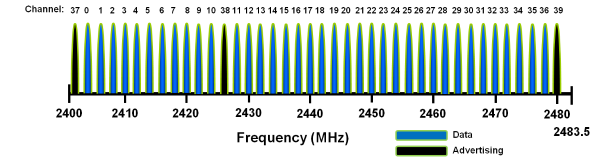
\includegraphics[width = 1\textwidth]{image/ble-phy-channel-assignment.png}
    \caption{廣播頻道與資料頻道示意圖\cite{microchip2023}}
    \label{fig: 廣播頻道與資料頻道示意圖}
\end{figure*}

廣播模式和連接模式的運作機制由 BLE 的控制層(Controller Layer)狀態機管理,包括Standby(等待)、Advertising(廣播)、Scanning(掃描)、Initiating(初始化)、Connection(連接)五種狀態 ,如圖(2.2)所示。

\begin{figure*}[htbp]
    \centering
    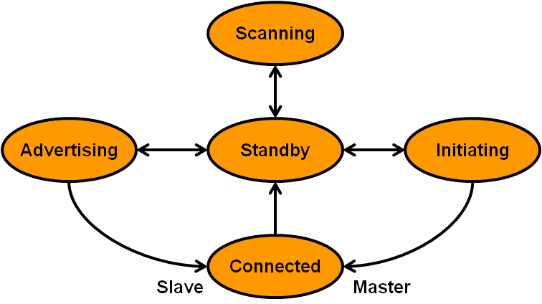
\includegraphics[width = 1\textwidth]{image/ble-link-layer-sm.png}
    \caption{Controller layer 狀態機示意圖\cite{microchip2023}}
    \label{fig: Controller layer 狀態機示意圖}
\end{figure*}


\subsection{廣播模式 (Advertising Mode)}

在廣播模式中,會使用Channel 37、Channel 38、channel 39這三個廣播頻道,主要用於掃描裝置、建立通訊頻道和廣播的傳輸,其中廣播者(Advertiser)是由待機狀態(Standby Status)進入廣播狀態(Advertising Status),廣播者會在三個廣播頻道輪流發送廣播封包,讓掃描者(Scanner)可以檢測到其存在,並提供基本的數據,例如:裝置名稱或狀態。
掃描者(Scanner)是由待機狀態(Standby Status)進入掃描狀態(Scanner Status),掃描者會輪流掃描三個廣播頻道的廣播封包,已接收範圍內的所有廣播的資訊,掃描收集數據後,準備與廣播設備建立連接,如圖(2.3)所示。
\begin{figure*}[htbp]
    \centering
    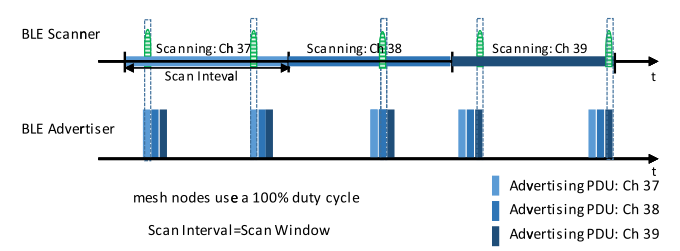
\includegraphics[width = 0.8\textwidth]{image/廣播模式示意圖.png}
    \caption{廣播模式示意圖\cite{9035389}}
    \label{fig: 廣播模式示意圖}
\end{figure*}




\subsection{連接模式 (Connection-Oriented Mode)}

連接模式中,設備需要首先透過廣播模式建立連接,其中廣播者(Slave)負責發送連線請求的廣播封包,而掃描者(Master)檢測到廣播封包後,從 Standby 進入 Scanning,再進入 Initiating 狀態,開始與廣播設備握手 (Handshake)。
當握手成功後,雙方進入 Connection 狀態。連接建立後,Master 與 Slave 可通過剩餘的 37 個數據頻道進行數據傳輸;Master 負責與多個 Slave 的連線管理,分配專屬的時間槽 (Time Slot) 給各連接設備,即使沒有數據需要傳輸,系統仍會保留固定的時間槽以確保系統的穩定性,避免通訊衝突。(圖2.4)為連線模式示意圖

\begin{figure*}[htbp]
    \centering
    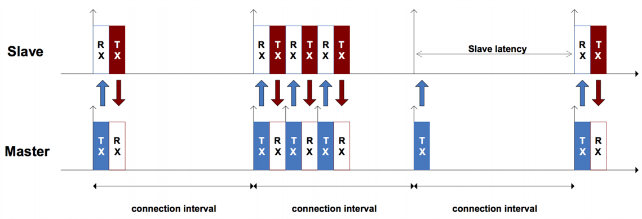
\includegraphics[width = 0.9\textwidth]{image/連線模式示意圖.png}
    \caption{連線模式示意圖\cite{9035389}}
    \label{fig: 連線模式示意圖}
\end{figure*}

\subsection{BLE排程機制}

廣播者(Advertiser)和掃描者(Scanner)會在建立連線後,進行數據的交換,當掃描者在三個掃描頻道掃瞄並偵測到廣播者發送的封包後,掃描者會在約 150 微秒($T_{IFS}$)後回應一個 CONNECT\_IND 封包。CONNECT\_IND 封包包含了多項管理連接的參數,例如:影響錨點時間(Anchor Point, AP)的 WinSize 以及 WinOffset。
建立連線之後,Connection Interval (CI)、Anchor Point (AP)和Connection Event (CE)對於裝置之間的排成機制影響非常的大,在一個Connection Interval(CI)的時間內,一個Slave裝置只會與Master裝置有一個Connection Event(CE)傳輸時間來進行資料的交換,所以Connection Interval(CI)的時間影響Connection Event(CE)的發生頻率,這直接影響到整個系統的效能及吞吐量,圖(2.5)表示了Master連接建立過程和連接事件。                                            
\begin{figure*}[htbp]
    \centering
    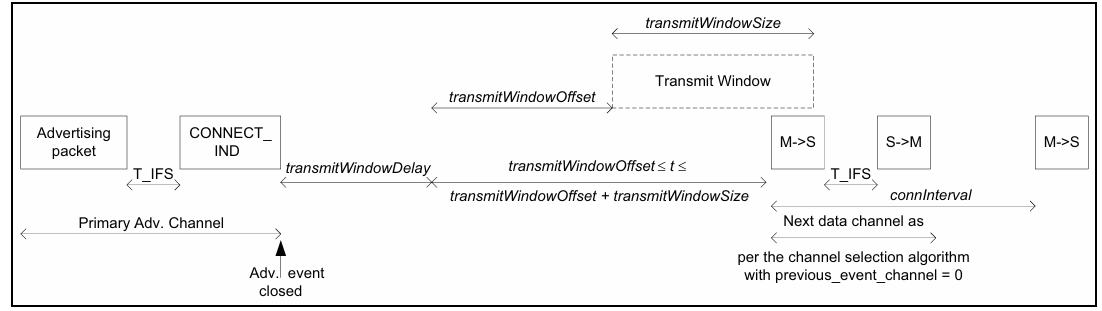
\includegraphics[width = 1\textwidth]{image/Master 連接建立過程和連接事件.png}
    \caption{Master 連接建立過程和連接事件\cite{bluetooth2016core}}
    \label{fig: Master 連接建立過程和連接事件}
\end{figure*}

\texttt{CONNECT\_IND} 封包會在 $t_{\mathrm{ind}}$ 時間內完成傳輸,Master 會在公式(a)至公式(b)的時間內設置第一個錨點(Anchor Point, AP),其中 transmitWindowDelay 通常為 $1.25\,\mathrm{ms}$,用來同步 Master 與 Slave。transmitWinOffset 與 transmitWinSize 分別由公式(c)與(d)算出。WinOffset代表錨點(Anchor Point, AP)的偏移量;WinSize代表錨點(Anchor Point, AP)可能發生的時間範圍\cite{10.1145/3412382.3458271}。

\begin{align}
t_{\mathrm{ind}} + \text{transmitWindowDelay} + \text{transmitWinOffset} \tag{a} \\
t_{\mathrm{ind}} + \text{transmitWindowDelay} + \text{transmitWinOffset} + \text{transmitWinSize} \tag{b} \\
\text{transmitWinOffset} = \text{WinOffset} \times 1.25\,\mathrm{ms} \tag{c} \\
\text{transmitWinSize} = \text{WinSize} \times 1.25\,\mathrm{ms} \tag{d}
\end{align}


\end{ZhChapter}